\documentclass{article}
%%%%%%%%%%%%%%%%%%%%%%%%%%%%%%%%%%%%%%%%%
% Lachaise Assignment
% Structure Specification File
% Version 1.0 (26/6/2018)
%
% This template originates from:
% http://www.LaTeXTemplates.com
%
% Authors:
% Marion Lachaise & François Févotte
% Vel (vel@LaTeXTemplates.com)
%
% License:
% CC BY-NC-SA 3.0 (http://creativecommons.org/licenses/by-nc-sa/3.0/)
% 
%%%%%%%%%%%%%%%%%%%%%%%%%%%%%%%%%%%%%%%%%

%----------------------------------------------------------------------------------------
%	PACKAGES AND OTHER DOCUMENT CONFIGURATIONS
%----------------------------------------------------------------------------------------

\usepackage{amsmath,amsfonts,stmaryrd,amssymb,subcaption} % Math packages

\usepackage{enumerate} % Custom item numbers for enumerations

\usepackage[ruled]{algorithm2e} % Algorithms

\usepackage[framemethod=tikz]{mdframed} % Allows defining custom boxed/framed environments

\usepackage{listings} % File listings, with syntax highlighting
\lstset{
	basicstyle=\ttfamily, % Typeset listings in monospace font
}

%----------------------------------------------------------------------------------------
%	DOCUMENT MARGINS
%----------------------------------------------------------------------------------------

\usepackage{geometry} % Required for adjusting page dimensions and margins

\geometry{
	paper=a4paper, % Paper size, change to letterpaper for US letter size
	top=2cm, % Top margin
	bottom=2.5cm, % Bottom margin
	left=2cm, % Left margin
	right=2cm, % Right margin
	headheight=14pt, % Header height
	footskip=1.5cm, % Space from the bottom margin to the baseline of the footer
	headsep=1.2cm, % Space from the top margin to the baseline of the header
	%showframe, % Uncomment to show how the type block is set on the page
}

%----------------------------------------------------------------------------------------
%	FONTS
%----------------------------------------------------------------------------------------

\usepackage[utf8]{inputenc} % Required for inputting international characters
\usepackage[T1]{fontenc} % Output font encoding for international characters

\usepackage{XCharter} % Use the XCharter fonts

%----------------------------------------------------------------------------------------
%	COMMAND LINE ENVIRONMENT
%----------------------------------------------------------------------------------------

% Usage:
% \begin{commandline}
%	\begin{verbatim}
%		$ ls
%		
%		Applications	Desktop	...
%	\end{verbatim}
% \end{commandline}

\mdfdefinestyle{commandline}{
	leftmargin=10pt,
	rightmargin=10pt,
	innerleftmargin=15pt,
	middlelinecolor=black!50!white,
	middlelinewidth=2pt,
	frametitlerule=false,
	backgroundcolor=black!5!white,
	frametitle={Command Line},
	frametitlefont={\normalfont\sffamily\color{white}\hspace{-1em}},
	frametitlebackgroundcolor=black!50!white,
	nobreak,
}

% Define a custom environment for command-line snapshots
\newenvironment{commandline}{
	\medskip
	\begin{mdframed}[style=commandline]
}{
	\end{mdframed}
	\medskip
}

%----------------------------------------------------------------------------------------
%	FILE CONTENTS ENVIRONMENT
%----------------------------------------------------------------------------------------

% Usage:
% \begin{file}[optional filename, defaults to "File"]
%	File contents, for example, with a listings environment
% \end{file}

\mdfdefinestyle{file}{
	innertopmargin=1.6\baselineskip,
	innerbottommargin=0.8\baselineskip,
	topline=false, bottomline=false,
	leftline=false, rightline=false,
	leftmargin=2cm,
	rightmargin=2cm,
	singleextra={%
		\draw[fill=black!10!white](P)++(0,-1.2em)rectangle(P-|O);
		\node[anchor=north west]
		at(P-|O){\ttfamily\mdfilename};
		%
		\def\l{3em}
		\draw(O-|P)++(-\l,0)--++(\l,\l)--(P)--(P-|O)--(O)--cycle;
		\draw(O-|P)++(-\l,0)--++(0,\l)--++(\l,0);
	},
	nobreak,
}

% Define a custom environment for file contents
\newenvironment{file}[1][File]{ % Set the default filename to "File"
	\medskip
	\newcommand{\mdfilename}{#1}
	\begin{mdframed}[style=file]
}{
	\end{mdframed}
	\medskip
}

%----------------------------------------------------------------------------------------
%	NUMBERED QUESTIONS ENVIRONMENT
%----------------------------------------------------------------------------------------

% Usage:
% \begin{question}[optional title]
%	Question contents
% \end{question}

\mdfdefinestyle{question}{
	innertopmargin=1.2\baselineskip,
	innerbottommargin=0.8\baselineskip,
	roundcorner=5pt,
	nobreak,
	singleextra={%
		\draw(P-|O)node[xshift=1em,anchor=west,fill=white,draw,rounded corners=5pt]{%
		Question \theQuestion\questionTitle};
	},
}

\newcounter{Question} % Stores the current question number that gets iterated with each new question

% Define a custom environment for numbered questions
\newenvironment{question}[1][\unskip]{
	\bigskip
	\stepcounter{Question}
	\newcommand{\questionTitle}{~#1}
	\begin{mdframed}[style=question]
}{
	\end{mdframed}
	\medskip
}

%----------------------------------------------------------------------------------------
%	WARNING TEXT ENVIRONMENT
%----------------------------------------------------------------------------------------

% Usage:
% \begin{warn}[optional title, defaults to "Warning:"]
%	Contents
% \end{warn}

\mdfdefinestyle{warning}{
	topline=false, bottomline=false,
	leftline=false, rightline=false,
	nobreak,
	singleextra={%
		\draw(P-|O)++(-0.5em,0)node(tmp1){};
		\draw(P-|O)++(0.5em,0)node(tmp2){};
		\fill[black,rotate around={45:(P-|O)}](tmp1)rectangle(tmp2);
		\node at(P-|O){\color{white}\scriptsize\bf !};
		\draw[very thick](P-|O)++(0,-1em)--(O);%--(O-|P);
	}
}

% Define a custom environment for warning text
\newenvironment{warn}[1][Warning:]{ % Set the default warning to "Warning:"
	\medskip
	\begin{mdframed}[style=warning]
		\noindent{\textbf{#1}}
}{
	\end{mdframed}
}

%----------------------------------------------------------------------------------------
%	INFORMATION ENVIRONMENT
%----------------------------------------------------------------------------------------

% Usage:
% \begin{info}[optional title, defaults to "Info:"]
% 	contents
% 	\end{info}

\mdfdefinestyle{info}{%
	topline=false, bottomline=false,
	leftline=false, rightline=false,
	nobreak,
	singleextra={%
		\fill[black](P-|O)circle[radius=0.4em];
		\node at(P-|O){\color{white}\scriptsize\bf i};
		\draw[very thick](P-|O)++(0,-0.8em)--(O);%--(O-|P);
	}
}

% Define a custom environment for information
\newenvironment{info}[1][Info:]{ % Set the default title to "Info:"
	\medskip
	\begin{mdframed}[style=info]
		\noindent{\textbf{#1}}
}{
	\end{mdframed}
}
 % Include the file specifying the document structure and custom commands
\setlength\parindent{0pt}
\usepackage[]{algorithm2e}
\usepackage{algpseudocode}

\title{EECS 545: Homework \#4} % Title of the assignment

\author{Mingliang Duanmu\\ \texttt{duanmuml@umich.edu}} % Author name and email address

\date{\today} % University, school and/or department name(s) and a date

\begin{document}

\maketitle % Print the title

\section{Neural Network Layer Implementation}

\subsection*{Fully-Connected Layer}

$$\frac{\partial Y_m^{(n)}}{\partial W_{ij}} = \frac{\partial}{\partial W_{ij}} (\sum_l W_{nl}X_{lm} + b_m) = X_{nj}\delta_{ni}\delta_{mj}$$
$$\frac{\partial Y_m^{(n)}}{\partial b_j} = \frac{\partial}{\partial b_j} (\sum_l W_{nl}X_{lm} + b_m) = \delta_{mj}$$
$$\frac{\partial Y_m^{(n)}}{\partial X_{ij}} = \frac{\partial}{\partial X_{ij}} (\sum_l W_{nl}X_{lm} + b_m) = W_{nj}\delta_{ni}\delta_{mj}$$
where $\delta_{ij}$ is Kronecker Delta, $\delta_{ij} = 1$ if $i=j$, else $0$. By vectorizing the result, we get
$$\frac{\partial L}{\partial W} = \frac{\partial L}{\partial Y}\frac{\partial Y}{\partial W} = \frac{\partial L}{\partial Y} X^T$$
$$\frac{\partial L}{\partial b} = \frac{\partial L}{\partial Y}\frac{\partial Y}{\partial b} = \sum_i \frac{\partial L}{\partial Y_i}$$
$$\frac{\partial L}{\partial X} = \frac{\partial L}{\partial Y}\frac{\partial Y}{\partial X} = W^T \frac{\partial L}{\partial Y}$$

\subsection*{ReLU}

$$\frac{\partial L}{\partial X} = \frac{\partial L}{\partial Y}\frac{\partial Y}{\partial X} = \frac{\partial L}{\partial Y} \circ \Delta(X)$$
where $\circ$ is element-wise product and $\Delta(X)_{ij} = I(x_{ij} > 0)$.

\newpage

\section{Multi-class classification with Softmax}

\texttt{hidden\_dim} = 80, \texttt{accuracy} = 0.9695 \\
\texttt{hidden\_dim} = 100, \texttt{accuracy} = 0.9698 \\
\texttt{hidden\_dim} = 128, \texttt{accuracy} = 0.9697 \\
\texttt{hidden\_dim} = 192, \texttt{accuracy} = 0.9678 \\
\texttt{hidden\_dim} = 200, \texttt{accuracy} = 0.972 \\
\texttt{hidden\_dim} = 256, \texttt{accuracy} = 0.97
\begin{figure}[htbp]
    \centering
    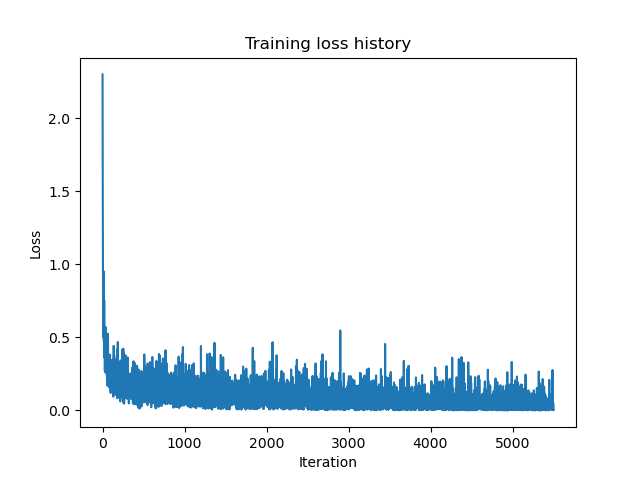
\includegraphics[width=.7\textwidth]{softmax_loss.png}
\end{figure}

\newpage

\section{Convolutional Neural Network for multi-class classification}

\texttt{accuracy} = 0.9803
\begin{figure}[htbp]
    \centering
    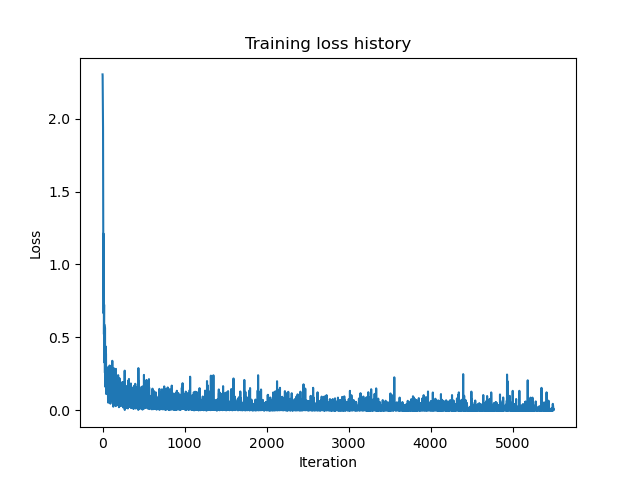
\includegraphics[width=.7\textwidth]{cnn_loss.png}
\end{figure}

\newpage

\section{Application to Image Captioning}

\begin{figure}[htbp]
    \centering
    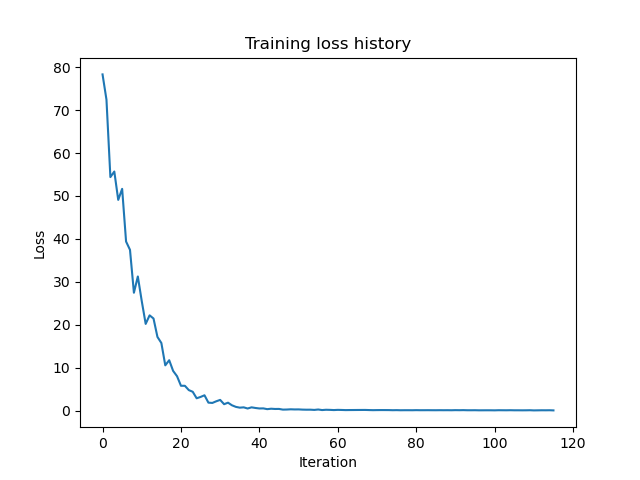
\includegraphics[width=.5\textwidth]{ic_loss.png}
\end{figure}
\begin{figure}[htbp]
    \begin{subfigure}{.5\textwidth}
        \centering
        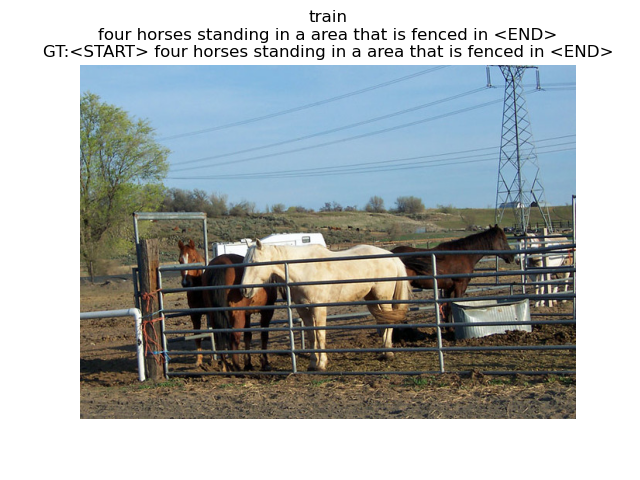
\includegraphics[width=.88\linewidth]{Figure_1.png}  
    \end{subfigure}
    \begin{subfigure}{.5\textwidth}
      \centering
      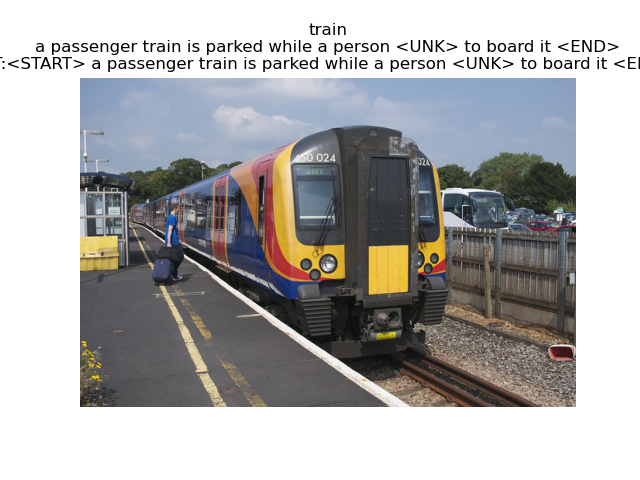
\includegraphics[width=.88\linewidth]{Figure_2.png}
    \end{subfigure}
    \begin{subfigure}{.5\textwidth}
        \centering
        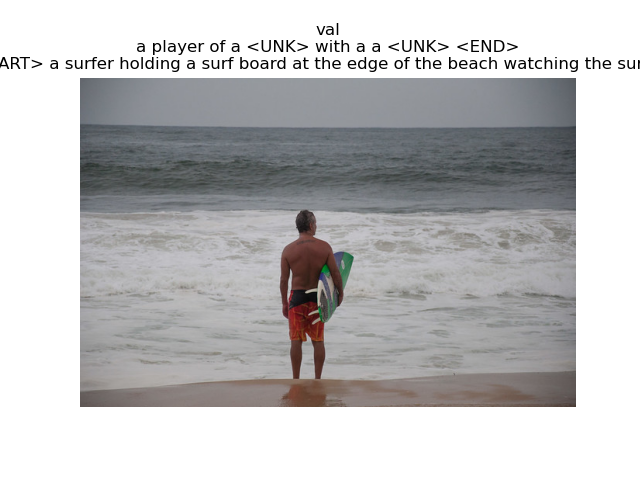
\includegraphics[width=.88\linewidth]{Figure_3.png}  
    \end{subfigure}
    \begin{subfigure}{.5\textwidth}
      \centering
      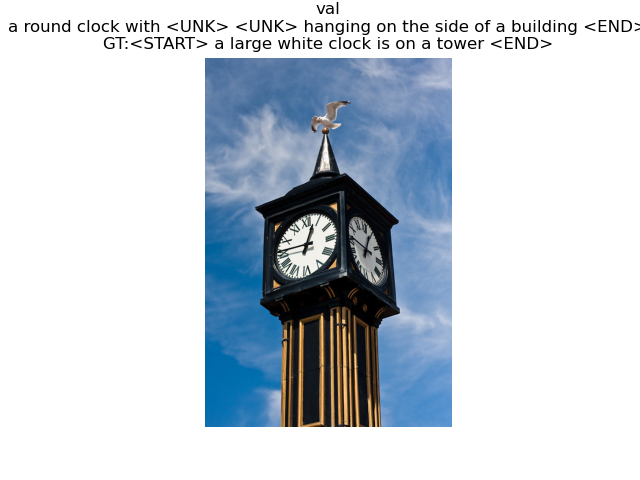
\includegraphics[width=.88\linewidth]{Figure_4.png}
    \end{subfigure}
\end{figure}

\newpage

\section{Transfer Learning}

Finetune the pre-trained model: \texttt{accuracy} = 0.954248 \\
Freeze the parameters in pre-trained model and train the final fc layer: \texttt{accuracy} = 0.960784
 
\end{document}